Di seguito viene spiegato come utilizzare le principali funzionalità dell'applicativo con l'ausilio di immagini.

\subsection{Ricerca di un progetto}

È possibile fare ricerche di progetti utilizzando come filtro l'username di un utente oppure il nome di un progetto.
\newline
Per eseguire una ricerca è sufficiente recarsi sulla home page tramite l'utilizzo del pulsante \textbf{PREMI} posto nell'angolo superiore sinistro dello schermo, scrivere la chiave di ricerca nell'apposita casella di testo, selezionare il filtro che si vuole utilizzare (Users o Project) e infine premere il tasto \textbf{Search}.

\begin{figure}[h] 
	\centering 
	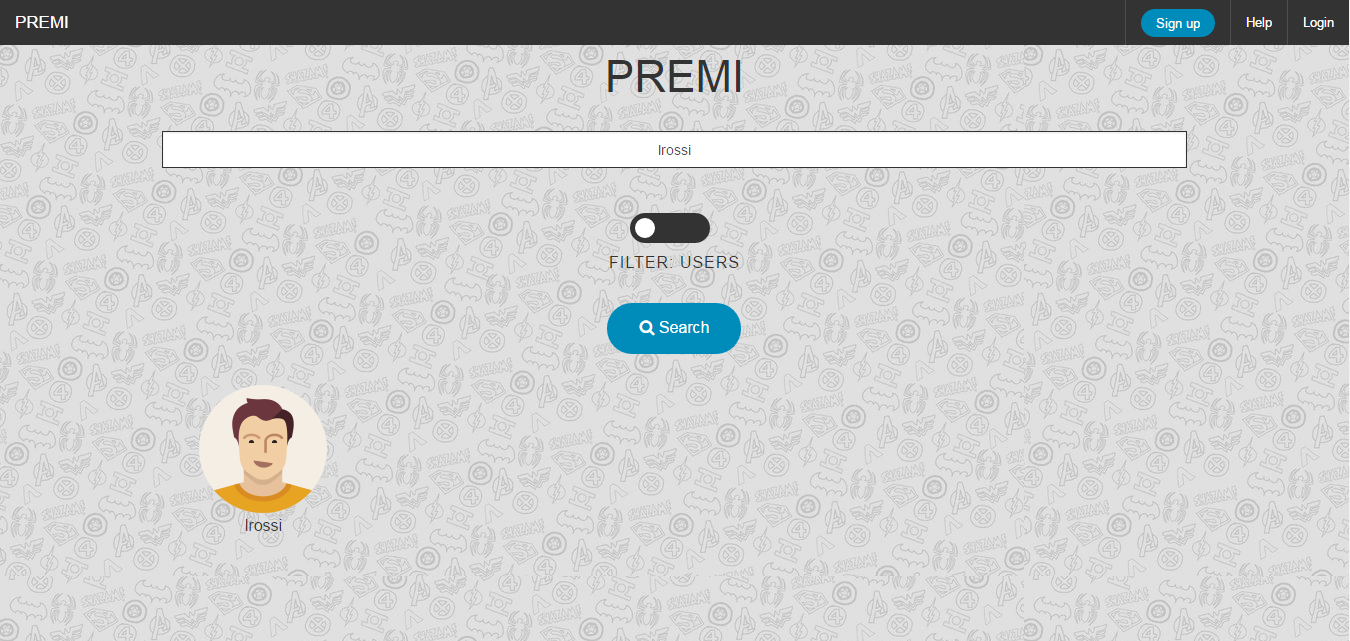
\includegraphics[scale=0.40] {img/ricerca.png}
	\caption{Ricerca} 
\end{figure}


\noindent I risultati della ricerca verranno mostrati sotto il pulsante \textbf{Search}, come mostrato nella figura sottostante.

\begin{figure}[h] 
	\centering 
	
\includegraphics[scale=0.40] {img/ricercaris.png}
	\caption{Risultati ricerca} 
\end{figure}

\newpage
\subsection{Registrazione}
Per creare un nuovo account utente è necessario premere il pulsante \textbf{Sign Up} posto nell'angolo superiore destro dello schermo. Si aprirà un pop-up nel quale saranno richieste le informazioni necessarie per registrare il nuovo utente (tutti i campi dati sono obbligatori). Dopo aver inserito i propri dati è sufficiente premere il tasto \textbf{Confirm}.

\begin{figure}[h] 
	\centering 
	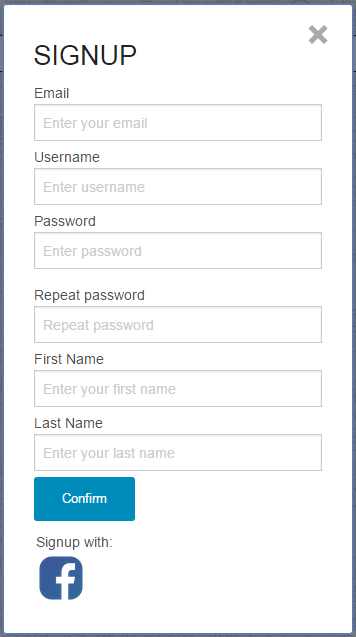
\includegraphics[scale=0.40] {img/signup.png}
	\caption{Registrazione} 
\end{figure}

\noindent Nel caso in cui tutti i dati inseriti siano stati accettati, il sistema effettuerà in automatico il login del nuovo utente creato reindirizzandolo alla sua pagina personale.
In caso contrario verranno segnalati i campi dati da correggere.

\subsection{Autenticazione}
Se un utente è già in possesso di un account e vuole autenticarsi è necessario premere il pulsante \textbf{Login} posto nell'angolo superiore destro dello schermo, infine inserire il proprio username, la password e premere \textbf{OK}.

\begin{figure}[h] 
	\centering 
	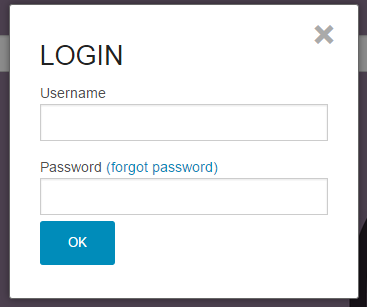
\includegraphics[scale=0.40] {img/login.png}
	\caption{Login} 
\end{figure}

\noindent Se i dati inseriti sono corretti il sistema reindirizzerà l'utente alla propria pagina personale, altrimenti verrà segnalato un errore nelle credenziali inserite.
\newline
\noindent Nel caso in cui l'utente non ricordi più la sua password, può premere il link \textit{Forgot password}. Una volta premuto si aprirà un pop-up nel quale verrà richiesto di inserire la mail utilizzata al momento della registrazione al fine di recuperare la password di accesso. Dopo aver inserito la mail corretta e aver premuto \textbf{Submit} la procedura di recupero password sarà inviata alla mail indicata. Il pop-up è mostrato nella figura sottostante.

\begin{figure}[H] 
	\centering 
	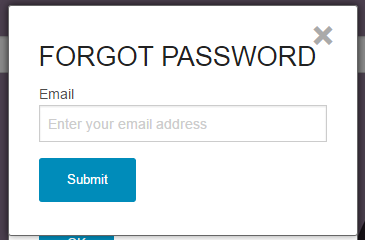
\includegraphics[scale=0.40] {img/forgot.png}
	\caption{Recupero password} 
\end{figure}

\subsection{Pagina personale}
Una volta autenticato un utente ha accesso alla sua pagina personale, nella quale sono riportati tutti i dati relativi a esso e dalla quale può accedere a tutte le funzionalità del sistema.

\begin{figure}[H] 
	\centering 
	\includegraphics[scale=0.40] {img/myaccount.png}
	\caption{Pagina personale} 
\end{figure}

\subsection{Logout}
Un utente autenticato può eseguire il logout, da qualunque pagina stia visualizzando, tramite il pulsante \textbf{Logout} posto nell'angolo in alto a destro dello schermo.

\begin{figure}[H] 
	\centering 
	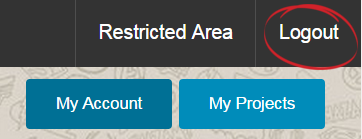
\includegraphics[scale=0.80] {img/logout.png}
	\caption{Logout} 
\end{figure}
